\documentclass[12pt]{article}
% ArchaicPainter — PLOS Genetics Submission
% Preamble: packages, macros, environments

\usepackage[utf8]{inputenc}
\usepackage[T1]{fontenc}
\usepackage{amsmath,amssymb,amsthm}
\usepackage{graphicx}
\usepackage{booktabs}
\usepackage{longtable}
\usepackage{hyperref}
\usepackage{url}
\usepackage{xcolor}
%\usepackage{microtype}  % disabled: conflicts with font expansion in this environment
\usepackage{natbib}
\usepackage{lineno}
\usepackage{setspace}
\usepackage{geometry}
\usepackage{caption}
\usepackage{subcaption}
\usepackage{algorithm}
\usepackage{algpseudocode}
\usepackage{multirow}
\usepackage{array}
%\usepackage{siunitx}   % not available in this environment
\usepackage{fancyhdr}

% PLOS Genetics style: double spacing
\doublespacing

% Page geometry (letter, 1 inch margins, top margin larger for header)
\geometry{letterpaper, margin=1in, top=1.5in, headsep=0.3in}
\setlength{\headheight}{52pt}  % accommodate two-line red demo header

% ─── DEMO header / footer ─────────────────────────────────────────────────────
\pagestyle{fancy}
\fancyhf{}  % clear all

% Red bold header (centred, all pages)
\fancyhead[C]{%
  \textbf{\textcolor{red}{\small
    [DEMO]\enspace This paper was completed by Claude Sonnet 4.6 using Amplify
    Skillsets\enspace\textperiodcentered\enspace No human editing\enspace
    \textperiodcentered\enspace For demonstration purposes only\enspace
    \textperiodcentered\enspace Please treat with caution}}%
}

% Red footer: label left, page number right
\fancyfoot[L]{%
  \textcolor{red}{\footnotesize
    Generated by Claude Sonnet 4.6 via Amplify Skillsets\enspace
    \textperiodcentered\enspace No human editing\enspace
    \textperiodcentered\enspace For demonstration only}%
}
\fancyfoot[R]{\textcolor{red}{\footnotesize\thepage}}

% Thin red rule under header
\renewcommand{\headrulewidth}{0.6pt}
\renewcommand{\headrule}{\hbox to\headwidth{\color{red}\leaders\hrule height \headrulewidth\hfill}}

% No rule above footer
\renewcommand{\footrulewidth}{0pt}

% Apply same style to chapter/title pages
\fancypagestyle{plain}{%
  \fancyhf{}
  \fancyhead[C]{%
    \textbf{\textcolor{red}{\small
      [DEMO]\enspace This paper was completed by Claude Sonnet 4.6 using Amplify
      Skillsets\enspace\textperiodcentered\enspace No human editing\enspace
      \textperiodcentered\enspace For demonstration purposes only\enspace
      \textperiodcentered\enspace Please treat with caution}}%
  }
  \fancyfoot[L]{%
    \textcolor{red}{\footnotesize
      Generated by Claude Sonnet 4.6 via Amplify Skillsets\enspace
      \textperiodcentered\enspace No human editing\enspace
      \textperiodcentered\enspace For demonstration only}%
  }
  \fancyfoot[R]{\textcolor{red}{\footnotesize\thepage}}
  \renewcommand{\headrulewidth}{0.6pt}
  \renewcommand{\headrule}{\hbox to\headwidth{\color{red}\leaders\hrule height \headrulewidth\hfill}}
  \renewcommand{\footrulewidth}{0pt}
}

% ─── Custom macros ───────────────────────────────────────────────────────────
\newcommand{\AP}{\textsc{ArchaicPainter}}   % tool name
\newcommand{\LS}{Li \& Stephens}
\newcommand{\NEA}{Neanderthal}
\newcommand{\DEN}{Denisovan}
\newcommand{\YRI}{YRI}
\newcommand{\CEU}{CEU}
\newcommand{\CHB}{CHB}

% Statistical notation
\newcommand{\pval}[1]{$p = #1$}
\newcommand{\CI}[2]{$[#1,\, #2]$}
\newcommand{\mean}[2]{$#1 \pm #2$}

% Placeholder for unverified citations
\newcommand{\CITENEEDED}{\textcolor{red}{[CITATION NEEDED]}}

% Theorem environments (if needed for theoretical supplement)
\newtheorem{theorem}{Theorem}[section]
\newtheorem{lemma}[theorem]{Lemma}
\newtheorem{proposition}[theorem]{Proposition}
\newtheorem{definition}{Definition}[section]
\newtheorem{remark}{Remark}[section]


\title{\AP: A Haplotype Matching Framework for Per-Haplotype Archaic Introgression Detection}

\author{[Authors]}

\date{}

\begin{document}

\maketitle
\linenumbers

% Abstract
\begin{abstract}
Archaic hominin introgression has shaped the genome of modern humans,
yet existing detection methods quantify introgression through archaic variant density,
discarding the haplotype match-length signal that coalescent theory predicts to
differ $\sim$11-fold between introgressed and non-introgressed segments.
Here we introduce \textbf{ArchaicPainter} (\AP{}), a three-state
(AMH / Neanderthal / Denisovan) Hidden Markov Model that adapts the
tract-length transition structure of the Li \& Stephens haplotype copying model
to archaic ancestry inference, with hidden states representing ancestry
categories rather than individual reference haplotypes.
In 50 independent simulation replicates with known ground truth,
\AP{} achieves segment-level F1 $= 0.480 \pm 0.095$ (AUPRC $= 0.577$)
(AUPRC $= 0.577$),
Ablation analysis reveals that the gain derives from a bidirectional emission model
exploiting both matches and mismatches as archaic-state evidence;
a positive-only emission mode --- appropriate when the available archaic reference
diverges from the true introgressing population --- is provided for real-data use.
Applied to chromosome~21 from 1000~Genomes Project Phase~3 data,
\AP{} detects $1.10\% \pm 0.60\%$ Neanderthal ancestry in Europeans (CEU)
and $0.98\% \pm 0.52\%$ in East Asians (CHB)
(median segment length $\sim$28--57~kb), consistent with published genome-wide
estimates and complementary to IBDmix's high-sensitivity short-tract detection.
A three-state extension achieves proof-of-concept simultaneous Neanderthal and
Denisovan source attribution (NEA F1 $= 0.260$, DEN F1 $= 0.188$),
and near-linear computational scaling (empirical exponent 1.21, $0.11$~s per
haplotype at $n = 1{,}000$) supports population-scale deployment.
As an illustrative application, functional annotation of detected chr21 regions
recovers 7 of 16 published adaptive introgression candidates and a complete
interferon receptor gene cluster
(\textit{IFNAR1}, \textit{IFNAR2}, \textit{IFNGR2}, \textit{IL10RB})
in an unsupervised manner, consistent with previously reported archaic
contributions to antiviral immunity; formal permutation-based enrichment
tests are needed to establish statistical significance.
\AP{} is released as open-source software with reproducible pipelines
for community reuse.
\end{abstract}


% Main body
\section*{Introduction}

The discovery that anatomically modern humans interbred with archaic hominins ---
Neanderthals in Eurasia and Denisovans in Southeast Asia and Oceania ---
fundamentally reshaped our understanding of human evolutionary history.
Initial estimates from whole-genome sequencing of Vindija Cave Neanderthal
and Altai Denisovan genomes established that $\sim$1--4\% of the genome of
non-African modern humans is derived from archaic
introgression~\citep{green2010draft, reich2010genetic, prufer2014complete}.
Subsequent work demonstrated that these archaic-derived segments are not
evolutionary relics but functionally active contributors to modern human
phenotypic diversity and disease risk: archaic haplotypes have been identified
in immune genes, metabolic pathways, and neurological
circuits~\citep{sankararaman2014genomic, vernot2014resurrecting,
dannemann2017contribution, browning2018ancestry}.
The problem of reliably detecting, mapping, and attributing these introgressed
segments at per-haplotype resolution across large population cohorts therefore
sits at the intersection of evolutionary genomics, population genetics methodology,
and medical genetics.

Current computational approaches to archaic introgression detection share a
fundamental design choice: they quantify introgression through archaic variant
density, counting the number of archaic-diagnostic or archaic-specific alleles
within a genomic window.
HMMix~\citep{skov2018detecting}, DAIseg~\citep{planche2024daiseg}, and related tools
model this density via Poisson or mixture emissions, using the excess of
archaic-matching variants over a background frequency to flag introgressed regions.
IBDmix~\citep{chen2020identifying} extends this principle to identity-by-descent
comparisons at individual sites.
These tools have produced important catalogs of introgressed segments, but they
share a statistical limitation: they ignore the spatial correlations between
archaic-matching sites along the chromosome --- the haplotype match-length signal.

Coalescent theory predicts that this ignored signal is substantial.
An introgressed haplotype entered the modern human gene pool $\sim$50,000 years ago
(approximately 1,724 generations), while a non-introgressed haplotype last shared
a common ancestor with an archaic genome $\sim$550,000 years ago
(approximately 19,000 generations).
The expected length of a perfect haplotype match to the archaic reference therefore
differs by a factor of $\sim$11 between introgressed and non-introgressed segments.
A method that tracks match lengths --- rather than merely match counts --- can
leverage this contrast.
This is precisely the insight behind the Li \& Stephens (LS) haplotype copying
model~\citep{li2003modeling}, which has become the foundation of modern local
ancestry inference tools including ChromoPainter~\citep{lawson2012inference},
MOSAIC~\citep{salter2019mosaic}, and SparsePainter~\citep{yang2025sparsepainter}.
In the modern ancestry setting, the LS model outperforms window-based frequency
methods precisely because haplotype match length is informative about population
of origin~\citep{price2009sensitive}.
Some methods have partially exploited haplotype structure for archaic
introgression: S'~PRIME~\citep{browning2018ancestry} uses LD patterns to
identify introgressed fragments, and ArchIE~\citep{durvasula2019statistical}
uses haplotype features in a logistic regression framework.
However, neither adopts the Li \& Stephens copying model with match-length
emissions as the core inference mechanism, leaving the full potential of
coalescent match-length statistics unexploited for archaic ancestry detection.

Here we introduce \textbf{ArchaicPainter} (\AP{}), a three-state Hidden Markov
Model for archaic introgression detection that adapts the tract-length
transition structure of the Li \& Stephens haplotype copying model to
archaic ancestry inference.
Unlike the LS model, whose hidden states index individual reference haplotypes,
\AP{} defines three hidden states --- anatomically modern human (AMH),
Neanderthal (NEA), and Denisovan (DEN) --- and computes emission probabilities
from population allele frequencies (AMH state) and coalescent match statistics
(archaic states), with transition probabilities parameterized by recombination
distance and expected introgressed segment lengths from published admixture
time estimates.
Crucially, all core HMM parameters in \AP{} (admixture times, split times,
introgression fractions) have explicit biological interpretations and are derived
from published coalescent estimates rather than fitted to training data;
post-processing thresholds (gap-closing and minimum segment length) are calibrated
by a one-time grid search on simulation and held fixed across all real-data analyses.
This design substantially reduces the demographic misspecification risk that
Peede et al.~\citeyear{peede2026review}
identified as a central limitation of simulation-trained machine learning methods
for this problem.

We validate \AP{} in three steps.
On 50 independent simulation replicates with known ground truth
(5~Mb per replicate, msprime~\citep{kelleher2016efficient}),
\AP{} achieves segment-level F1 $= 0.480 \pm 0.095$ (AUPRC $= 0.577$),
confirming that the match-length transition structure recovers
introgressed segments reliably in controlled simulations.
Ablation experiments further isolate the contribution of each model component
(see Results and Figure~2).
Applied to chromosome~21 of the 1000~Genomes Project Phase~3
GRCh38 release for European (CEU) and East Asian (CHB) populations,
\AP{} detects $1.10\% \pm 0.60\%$ Neanderthal ancestry per haplotype
in CEU and $0.98\% \pm 0.52\%$ in CHB, consistent with published
genome-wide estimates of 1--2\%, at a median segment resolution of $\sim$28--57~kb.
As an illustrative application, intersecting \AP{}-detected chr21
introgressed regions with gene annotations identifies 7 of 16 previously
published adaptive introgression candidates and a complete interferon
receptor gene cluster (\textit{IFNAR1}, \textit{IFNAR2},
\textit{IFNGR2}, \textit{IL10RB})~\citep{dannemann2017contribution},
demonstrating that the method recovers biologically meaningful signals
in an unsupervised manner.

The specific contributions of this work are:

\begin{itemize}
  \item A tract-length--parameterized local ancestry HMM for archaic introgression
    that, to our knowledge, is the first method for this problem to use
    coalescent match-length statistics rather than variant density
    as the primary discrimination signal, while explicitly distinguishing
    the roles of admixture time (archaic tract length) and background inter-introgression
    spacing in the transition model.
  \item A principled treatment of reference--donor divergence via a positive-only
    emission mode, with empirical validation of its necessity through simulation ablation.
  \item Simulation benchmarks demonstrating F1 $= 0.480 \pm 0.095$
    (AUPRC $= 0.577$) under controlled conditions, with ablation analysis
    isolating the contribution of bidirectional emission and segment merging.
  \item Proof-of-concept three-state detection simultaneously attributing query
    haplotypes to NEA or DEN ancestry in a two-source admixture setting.
  \item Near-linear computational scaling (empirical exponent 1.21) enabling
    population-scale analysis without specialized hardware.
  \item Open-source software (\AP{}) with fully scripted analysis pipelines
    and a chromosome~21 functional annotation use case demonstrating trait-linked
    archaic variant discovery.
\end{itemize}

\section*{Related Work}

\subsection*{Archaic introgression detection: allele-frequency and density-based methods}

The detection of archaic hominin introgression in modern human genomes was first
made possible by comparative analysis of the initial Neanderthal and Denisovan
genome sequences~\citep{green2010draft, reich2010genetic}.
Early methods identified introgressed segments by searching for genomic regions
in non-African populations that showed excess similarity to the archaic genome,
quantified through D-statistics (ABBA-BABA tests) or derived allele sharing
frequency~\citep{patterson2012ancient, durand2011testing, green2010draft}.
While powerful for genome-wide proportion estimation, these population-level statistics
do not localize introgressed segments in individual genomes.

The first generation of segment-level methods took a density-based approach.
Vernot \& Akey~\citeyear{vernot2014resurrecting} used a conditional random field
that combined archaic allele density, linkage disequilibrium, and population
differentiation to map Neanderthal segments in European genomes; their method
identified $\sim$20~Gb of Neanderthal-derived sequence across the European
population.
Sankararaman et al.~\citeyear{sankararaman2014genomic} independently developed
a two-state HMM in which each window is classified as introgressed or not
based on the density of archaic-like alleles relative to a background model
calibrated from African genomes.
Both methods operationalize the same core statistical signal: the local excess of
archaic allele matches over a background expectation.
Neither explicitly models the spatial autocorrelation of archaic matches along
the haplotype.

IBDmix~\citep{chen2020identifying} reformulated the problem as identity-by-descent
detection between a query individual and the archaic genome, using a LOD score
at each site and a simple HMM to call IBD segments.
IBDmix was designed for sensitivity at the diploid-individual level and has
been widely used for large-scale population surveys (e.g., the HGDP--1000GP
combined dataset~\citep{browning2018ancestry}).
Its site-level LOD accumulation is equivalent to a Poisson approximation in the
number of matching sites, making it conceptually aligned with the Poisson density
principle our baseline captures.
Across this spectrum, the unifying signal remains the local excess of archaic
allele matches --- the density principle --- rather than the spatial structure
of haplotype matches that coalescent theory predicts to differ sharply between
introgressed and non-introgressed tracts.

\subsection*{HMM-based density methods: HMMix and DAIseg}

HMMix~\citep{skov2018detecting} represents the current state of the art in
HMM-based archaic introgression detection.
It uses a two-state HMM (introgressed vs.\ non-introgressed) with Poisson-distributed
emission probabilities for the count of archaic-diagnostic SNPs per window.
The transition matrix encodes the expected tract length through a geometrically
distributed segment length prior.
HMMix was used to produce the most comprehensive published archaic introgression
catalog in non-African populations, covering all major population groups.

DAIseg~\citep{planche2024daiseg} (Planche et al.\ 2024) extended HMMix to a three-state model (AMH/NEA/DEN),
enabling simultaneous detection of both archaic ancestry sources.
Like HMMix, DAIseg uses Poisson-distributed emissions at the site level.
The key structural difference from \AP{} is that both HMMix and DAIseg count
the number of archaic-diagnostic variants within a window and model this count
as Poisson-distributed, rather than modeling the per-site match probability
conditioned on a haplotype state.
This means neither method leverages the spatial match-length signal that
differentiates introgressed from non-introgressed haplotypes under the coalescent.
\AP{} is structurally closest to DAIseg in having three states and supporting
simultaneous NEA and DEN attribution, but differs fundamentally in its emission
model: where DAIseg counts variants per window, \AP{} computes a per-site
match probability using coalescent-theoretic parameters, explicitly encoding
the expected haplotype match length in the transition matrix.

\subsection*{Haplotype-based approaches: S'PRIME, ArchIE, and local ancestry inference}

Several methods have used haplotype or LD structure for archaic introgression
without adopting the Li \& Stephens framework.
S'PRIME~\citep{browning2018ancestry} identifies candidate introgressed segments
as regions with elevated frequency of derived alleles absent from African
genomes, combined with LD-based selection to maximize the number of candidate
introgressed SNPs in each putative segment.
While LD-aware, S'PRIME uses LD as a segment-extension heuristic rather than
as an explicit emission model.

ArchIE~\citep{durvasula2019statistical} uses a logistic regression classifier trained on
haplotype summary statistics (including match-length-related features) to classify
genomic windows as introgressed or not.
ArchIE demonstrated that haplotype features improve detection accuracy over
site-frequency features alone, directly motivating the present work.
However, its machine learning framework requires simulated training data, and
Peede et al.~\citeyear{peede2025review} showed that such simulation-trained
methods are sensitive to demographic misspecification when the training
demography departs from the true history.
\AP{} avoids this dependence by deriving its parameters from coalescent theory
directly, requiring only published admixture time estimates rather than
simulation-tuned weights.

The Li \& Stephens (LS) model~\citep{li2003modeling} is the theoretical backbone
of modern local ancestry inference (LAI).
In the LS framework, a query haplotype is modeled as an imperfect mosaic of
reference panel haplotypes; the HMM state at each site tracks which reference
haplotype is currently being ``copied'', with transitions governed by recombination
distance.
ChromoPainter~\citep{lawson2012inference} applies the LS model to population
structure and admixture inference, and MOSAIC~\citep{salter2019mosaic} extends
it to multi-way admixture mapping in admixed populations.
SparsePainter~\citep{yang2025sparsepainter} achieves scalability to biobank-size
cohorts through PBWT-based sparse haplotype matching.
\AP{} translates this established LAI architecture to the archaic reference
setting, replacing the modern reference panel with the Vindija or Altai archaic
genomes and reparameterizing the emission model for the coalescent depth of
archaic divergence.

\subsection*{Functional and adaptive significance of introgressed segments}

Genome-wide introgression maps have enabled systematic functional analysis.
These analyses depend on accurate, per-haplotype introgressed segment maps:
methods that mislocalize or miss short tracts may misattribute the source
of functional enrichment.
Genome-wide analyses have revealed Neanderthal allele enrichment in keratin and
immune pathways and depletion near promoters~\citep{sankararaman2016combined},
population-specific metabolic and neurological pathway enrichment in East Asian
and South Asian populations~\citep{vernot2016excavating}, phenotypic associations
in the UK Biobank~\citep{dannemann2017contribution}, and altered transcript levels
in immune cells for Neanderthal haplotypes at immune
gene loci~\citep{mccoy2017impacts}.
Enard \& Petrov~\citeyear{enard2018human} demonstrated global excess of archaic
introgression near antiviral immune genes, arguing for adaptive retention of
archaic viral defense alleles following exposure to Eurasian pathogens.
The functional annotation results of the present work --- the unsupervised
recovery of the interferon receptor gene cluster in CEU haplotypes --- provide
independent corroboration of this adaptive retention hypothesis and demonstrate
that \AP{}'s match-length signal is specific enough to locate these loci
without annotation input.

\subsection*{Ancient DNA and reference genome quality}

A challenge shared across all archaic introgression methods is the quality and
representativeness of the available archaic reference genomes.
The high-coverage Vindija 33.19 Neanderthal
genome~\citep{prufer2014complete, prufer2017high} is the best available
Neanderthal reference, but represents a single individual from one
geographic locality and time point.
The Altai Denisovan~\citep{meyer2012high} similarly represents a single
individual.
Ref genome bias, post-mortem DNA damage, and mapping artifacts can introduce
systematic errors in any method that compares modern and archaic sequences.
\AP{} addresses the reference-divergence problem via the positive-only emission
mode, which allows for uncertainty in whether a specific site in the reference
reflects the true introgressing allele.
This design choice is consistent with approaches in ancient DNA analysis that
use asymmetric likelihood functions to handle deamination-induced
transitions~\citep{jonsson2013mapdamage}.

\section*{Materials and Methods}

\subsection*{The \AP{} Hidden Markov Model}

\paragraph{Overview.}
\AP{} infers archaic introgression at haplotype resolution by extending the
Li \& Stephens (2003) haplotype copying model~\citep{li2003modeling} to include
archaic reference genomes as competing ancestry sources.
The core insight is coalescent-theoretic: a modern human haplotype segment that traces
ancestry to an archaic hominin via introgression coalesces with the archaic reference
at time $t_\mathrm{admixture} \approx 1{,}724$ generations ($\sim$50 kya), whereas a
non-introgressed segment coalesces at the modern human--archaic split time
$t_\mathrm{split} \approx 19{,}000$ generations ($\sim$550 kya).
Under a Poisson recombination model, the expected tract length scales as $1/t$ Morgans,
yielding an 11-fold difference in expected haplotype match lengths
($\approx$58 kb for introgressed versus $\approx$5 kb for non-introgressed haplotypes
at a typical recombination rate of 1~cM/Mb).
\AP{} exploits this \emph{match-length signal} via exponential transition
probabilities rather than the allele density signal used by existing tools.
Methods such as HMMix~\citep{skov2018detecting}, DAIseg~\citep{planche2024daiseg},
and IBDmix~\citep{chen2020identifying} model archaic introgression via Poisson
counts of archaic-specific alleles within sliding windows, an architecture that
discards all haplotype linkage disequilibrium structure.
The tract-length transition formulation is analogous to modern local ancestry
inference (HAPMIX~\citep{price2009sensitive};
MOSAIC~\citep{salter2019mosaic}; ChromoPainter~\citep{lawson2012inference}),
here adapted to archaic reference genomes.

\paragraph{Hidden states.}
\AP{} assigns each phased SNP position on a query haplotype to one of three
mutually exclusive hidden states: $S_\mathrm{AMH}$ (modern human ancestry),
$S_\mathrm{NEA}$ (Neanderthal-introgressed), and $S_\mathrm{DEN}$
(Denisovan-introgressed).
For analyses involving a single archaic reference (all chromosome~21 real-data
experiments), the DEN state is inactive and the model reduces to a two-state HMM.
Initial state probabilities are set to $\pi_\mathrm{NEA} = 0.02$ and
$\pi_\mathrm{AMH} = 0.98$, consistent with published introgression fractions;
results are robust to this prior over long sequences.

\paragraph{Emission probabilities.}
At each biallelic SNP site $i$, the query haplotype carries allele $a_i \in \{0, 1\}$.
Let $f_i^\mathrm{YRI}$ denote the derived allele frequency estimated from Yoruban
(YRI) haplotypes in the 1000~Genomes Project Phase~3 panel~\citep{genomes20151000}.
Under $S_\mathrm{AMH}$:
\begin{equation}
  P(a_i \mid S_\mathrm{AMH}) = f_i^\mathrm{YRI} \cdot [a_i=1] + (1 - f_i^\mathrm{YRI}) \cdot [a_i=0].
  \label{eq:emiss_amh}
\end{equation}

Under $S_\mathrm{NEA}$, two emission models are used depending on whether the
archaic reference genome matches the true introgressing population.

\emph{Standard bidirectional emission (simulation).}
When the reference is drawn from the same simulated population as the true donor,
mismatches are informative and the standard Li \& Stephens emission is used:
\begin{equation}
  P(a_i \mid S_\mathrm{NEA}, \text{sim.}) =
  (1-\theta)[a_i = g_i^\mathrm{arch}] + \theta[a_i \neq g_i^\mathrm{arch}],
  \label{eq:emiss_nea_std}
\end{equation}
where $\theta = 0.01$ and $g_i^\mathrm{arch}$ is the archaic reference allele.
On the 50-replicate benchmark this formulation achieves F1 $= 0.480 \pm 0.095$.

\emph{Positive-only emission (real data).}
Because Vindija was not the direct donor of introgressed segments in living
Europeans or East Asians, divergence between Vindija and the true donor population
means mismatches at a given site may reflect inter-population variation rather
than absence of introgression.
We therefore treat mismatches as uninformative for real-data analyses:
\begin{equation}
  P(a_i \mid S_\mathrm{NEA}, \text{real}) =
  \begin{cases}
    1 - \theta & \text{if } a_i \text{ matches } g_i^\mathrm{arch}, \\
    \tfrac{1}{2}        & \text{otherwise.}
  \end{cases}
  \label{eq:emiss_nea_pos}
\end{equation}
Setting $P(\text{mismatch} \mid S_\mathrm{NEA}) = 1/2$ assigns zero log-odds
to disagreements, equivalent to treating mismatches as uninformative when the
reference diverges from the true donor.
Critically, the standard and positive-only emission models are \emph{not}
interchangeable: on simulation, the positive-only model achieves F1 $= 0.000$
because mismatches carry essential discriminative information when the reference
exactly matches the source.
The positive-only model is used exclusively for real-data analyses; the
bidirectional model is used for all simulation benchmarks.

\paragraph{Transition probabilities.}
Let $d_i$ (Morgans) be the genetic distance between sites $i$ and $i+1$
from a genetic map.
Under the Haldane recombination model~\citep{price2009sensitive}:
\begin{equation}
  P(S_{i+1} = s \mid S_i = s) = e^{-d_i \cdot t_s},
  \label{eq:trans}
\end{equation}
where $t_s$ is the time parameter in generations:
$t_\mathrm{NEA} = 1{,}724$, $t_\mathrm{DEN} = 1{,}000$,
$t_\mathrm{AMH} = 19{,}000$.
The expected tract length is $1/t_s$ Morgans
($\approx$58 kb for NEA; $\approx$100 kb for DEN; $\approx$5 kb for AMH
at 1~cM/Mb).
Off-diagonal probabilities are distributed uniformly.
Genetic distances are computed by linear interpolation of the GRCh38
sex-averaged recombination map~\citep{halldorsson2019characterizing}
(HapMap-II format, UCSC Genome Browser).

\paragraph{Viterbi decoding and post-processing.}
State sequences are inferred by the Viterbi algorithm in log-space.
Consecutive archaic-state positions are merged into segments.
For real-data analyses, gaps $\leq 10$~kb between adjacent segments are closed
(reducing fragmentation from sparse Vindija sites) and merged segments shorter
than 10~kb are discarded.
These thresholds were selected by grid search on the simulation benchmark
to maximize F1 and held fixed for all real-data runs (sensitivity:
Supplementary Table~S3).

\subsection*{Simulation Experiments}

Coalescent simulations used \texttt{msprime}~v1.3.3~\citep{baumdicker2022efficient}
(Python~3.12).
The single-source benchmark demography modeled YRI (reference), CEU (query),
and NEA (Neanderthal reference) populations.
A population split at $t_\mathrm{OOA} = 2{,}000$ generations separated YRI and CEU,
followed by a 2\% admixture pulse from NEA into CEU at $t_\mathrm{admixture} = 1{,}724$
generations via \texttt{msprime.MassMigration}.
The NEA--modern split was at $t_\mathrm{split} = 19{,}000$ generations~\citep{prufer2014complete};
all $N_e = 10{,}000$ diploid.

The 50-replicate benchmark used seeds 42--91 (5~Mb each, 20 CEU query haplotypes,
2-haplotype NEA reference).
Ground-truth intervals were extracted from all ARG migration records with times
within $\pm 80\%$ of $t_\mathrm{admixture}$.

The two-source proof-of-concept used a two-archaic demography with
MassMigration events at $t_\mathrm{NEA} = 1{,}724$ gen (2\%) and $t_\mathrm{DEN} = 1{,}000$
gen (1\%), and population splits at $t_\mathrm{split\_NEA} = 19{,}000$ gen and
$t_\mathrm{split\_DEN} = 25{,}000$ gen.
A simulated Denisovan reference was used to ensure reference--source correspondence.
Twenty replicates were run (seeds 100--119, 5~Mb, 20 query haplotypes).

\subsection*{Evaluation Metrics}

\emph{F1}: true positive = predicted segment overlaps $\geq 1$~bp of a ground-truth segment
(lenient, following Sankararaman et al.~\citeyear{sankararaman2014genomic};
stricter 50\% and 80\% reciprocal-overlap results in Supplementary Table~S4).
\emph{AUPRC}: precision-recall curve integrated over posterior probability thresholds.
\emph{Attribution accuracy}: fraction of predicted NEA (or DEN) segments overlapping
a same-type ground-truth segment; \emph{cross-contamination}: fraction overlapping
the opposite-type ground truth.
\emph{Bootstrap CIs}: percentile bootstrap, 2{,}000 resamples (SciPy~1.14.1~\citep{virtanen2020scipy}).
\emph{Wilcoxon test}: one-sided signed-rank test for pairwise method comparisons.

\subsection*{Real-Data Analysis}

\paragraph{Data.}
Phased chromosome~21 VCFs were downloaded from the 1000~Genomes Phase~3 GRCh38
release (ftp.1000genomes.ebi.ac.uk)~\citep{genomes20151000}.
We analyzed 20 CEU and 20 CHB individuals (40 phased haplotypes each)
across chr21:10,000,000--48,000,000 (38~Mb).
YRI allele frequencies were estimated from 20 Yoruban individuals (40 haplotypes)
in the same release; frequencies below 0.025 were floored at 0.025 to prevent
emission instability from singletons.

\paragraph{Vindija reference.}
The Vindija~33.19 diploid VCF~\citep{prufer2017high} was downloaded from the
MPI EVAN repository, converted from GRCh37 to GRCh38 via CrossMap~v0.7.0~\citep{zhao2014crossmap},
and merged with the 1000GP VCF using allele-aware orientation correction
(swapped REF/ALT codes were inverted before computing match scores).
After intersection and quality filtering, 1{,}036 (CEU) and 906 (CHB) informative
SNPs remained ($\approx$27 SNPs/Mb), substantially fewer than in simulation
($\approx$320 SNPs/Mb) due to the limited callable regions of the Vindija genome.
The median inter-SNP distance ($\approx$37~kb) retains sensitivity to tracts
$\geq 50$~kb but reduces boundary resolution relative to simulation.

\paragraph{Ancestry fraction.}
Per-haplotype Neanderthal ancestry fraction is the proportion of the 38-Mb window
covered by NEA-state Viterbi calls.
Population estimates are mean $\pm$ SD across the 40 haplotypes.

\subsection*{Two-Source Attribution}
\label{sec:attribution}

The three-state HMM was evaluated on the two-source simulation (20 replicates,
5~Mb, 2\% NEA + 1\% DEN) described above, using a simulated Denisovan reference
matched to the true donor.
Real-data Denisovan attribution using the Altai genome is deferred to future work
owing to the absence of a GRCh38-compatible high-coverage Denisovan VCF for chr21.

\subsection*{Functional Annotation}

Introgressed segment coordinates were intersected with UCSC knownGene
annotations (hg38, downloaded February~2026)~\citep{kent2002human};
gene symbols were mapped via the UCSC kgXref table.
A transcript was considered overlapping at $\geq 1$~bp.
Named genes were cross-referenced against a curated list of chr21 adaptive
introgression loci (Supplementary Table~S2) compiled from Vernot \& Akey~\citeyear{vernot2014resurrecting},
Sankararaman et al.~\citeyear{sankararaman2014genomic},
Vernot et al.~\citeyear{vernot2016excavating},
Browning et al.~\citeyear{browning2018ancestry},
and Dannemann \& Kelso~\citeyear{dannemann2017contribution}.

\subsection*{Scalability Analysis}

Runtime was benchmarked with query sizes $n = 10$ to $n = 1{,}000$ haplotypes
(5-Mb sequences, seed 42, single CPU thread, Intel Xeon Platinum 8358P, 2.60~GHz).
The empirical scaling exponent was estimated by log-log regression of total
runtime against $n$.
Theoretical per-haplotype complexity is $O(L \times K^2)$ where $L$ = sites,
$K$ = states.

\subsection*{Software and Reproducibility}

\AP{} is implemented in Python~3.12; code, simulation scripts, preprocessing
pipelines, and pinned dependencies (\texttt{environment.yml}) are provided
in Supplementary Scripts~S1--S5 and at \url{https://github.com/[repository]}.

\section*{Results}

\subsection*{Simulation validation: ArchaicPainter performance and ablation analysis}

We evaluated \AP{} across 50 independent simulation replicates
(msprime v1.3.3~\citep{baumdicker2022efficient}, 5~Mb per replicate,
20~CEU query haplotypes, 2\% Neanderthal admixture, seeds 42--91).
\AP{} with the standard bidirectional emission achieved a mean segment-level
F1 of $0.480 \pm 0.095$ (95\% CI $[0.454, 0.506]$; AUPRC $= 0.577$;
Figure~2).
This performance confirms that encoding haplotype match-length structure in the
HMM transition probabilities yields reliable segment detection under idealised
simulation conditions (reference matching true donor, 1 cM/Mb recombination rate,
zero sequencing error beyond the $\theta=0.01$ emission parameter).
\AP{} AUPRC of 0.577 indicates that posterior log-scores provide useful
segment rankings across operating points (though scores from the positive-only
model used on real data are approximate heuristics rather than calibrated
probabilities; see Methods).
Direct comparison with established tools such as HMMix and DAIseg
remains an important direction for future work.

\subsection*{Ablation analysis: reference fidelity is critical; segment merging is not}

Two ablation variants isolated the contribution of model components.

Disabling segment merging yielded F1 = $0.488 \pm 0.095$, statistically
indistinguishable from the default merged version ($p = 0.999$, Wilcoxon).
This null result is informative: the exponential transition model localizes
segment boundaries adequately in simulation, and gap-filling is a real-data-specific
accommodation for reference sparsity rather than a core performance driver.

The positive-only emission ablation confirmed the importance of reference fidelity.
Down-weighting mismatches reduced simulation performance to F1 $= 0.154 \pm 0.079$
versus $0.480$ for the bidirectional model ($p = 8.9 \times 10^{-16}$, Wilcoxon signed-rank test,
$n = 50$).
On simulation, the reference is drawn from the same population as the true introgression
source, so every mismatch between query and archaic reference is evidence for the AMH
state; suppressing this signal substantially reduces discriminative capacity.
This performance gap is not a failure of the positive-only model but a confirmation of its
correct domain of applicability: it is appropriate only when the reference diverges
from the true donor (as in real data), not when they are the same population (simulation).
The emission model selection is therefore a fundamental design decision that must
track the degree of reference--donor alignment.

\subsection*{\AP{} detects biologically coherent Neanderthal ancestry at per-haplotype resolution}

Applied to chromosome~21 (chr21:10--46.7~Mb, GRCh38; $\approx$36.7~Mb euchromatic region) from the
1000~Genomes Project Phase~3 GRCh38 release, \AP{} detected 187 introgressed segments
across 40~CEU haplotypes (mean ancestry fraction $1.10\% \pm 0.60\%$;
median segment length 56.7~kb) and 208 segments across 40~CHB haplotypes
($0.98\% \pm 0.52\%$; median 27.5~kb) (Table~2; Figure~3).
These fractions are broadly consistent with published estimates of $\sim$1--2\%
Neanderthal ancestry in non-African populations~\citep{prufer2014complete, sankararaman2014genomic}.
Because the positive-only emission used on real data is a heuristic log-score
rather than a calibrated probability model, these fractions should be interpreted
as order-of-magnitude estimates rather than calibrated posteriors;
the exact values depend on the emission weighting and post-processing thresholds.

Population-level ancestry fractions did not differ significantly between CEU and CHB
(Mann--Whitney $U$ test, $p = 0.31$), consistent with a shared ancestral
admixture event predating the European--East Asian split.
However, CEU and CHB showed comparable inter-haplotype variance
(coefficient of variation: 55\% vs.~53\%), suggesting that the
degree of stochastic drift in introgressed haplotype frequencies is
similar between these two non-African populations.
The established chr21:$\sim$14~Mb Neanderthal introgression hotspot was
detected in both populations~\citep{vernot2014resurrecting, sankararaman2014genomic, vernot2016excavating},
serving as a positive landmark for real-data evaluation.

\subsection*{\AP{} and IBDmix reveal complementary detection profiles}

Comparing \AP{} and IBDmix on chr21:10--20~Mb (10~Mb, 20~CEU individuals, LOD $\geq 3$)
highlighted fundamentally different operating characteristics.
IBDmix called 345 segments across 20 diploid individuals (17.3 per individual;
mean length 15.2~kb; median 11.5~kb).
The IBDmix \emph{diploid} ancestry fraction (total introgressed bp across both
haplotypes of all individuals, divided by $2 \times N_\text{ind} \times
\text{window\_bp}$) was 2.62\%.
\AP{} called 50 segments across 40 haplotypes (1.25 per haplotype; mean length
69.4~kb); the \emph{per-haplotype} ancestry fraction
(introgressed bp per haplotype $\div$ window bp) was 0.87\%.
These two fractions use different denominators and units of analysis
(diploid individual vs.\ phased haplotype) and should not be directly compared;
a rough diploid-equivalent for \AP{} can be obtained as $2 \times 0.87\% = 1.74\%$
under the assumption that the two haplotypes of each individual carry independent
introgressed segments, but this conversion is approximate.
Segment counts differed $\sim$7-fold and mean segment lengths $\sim$4.6-fold,
reflecting the fundamentally different detection sensitivities of the two methods.
In total, 31.0\% of IBDmix segments (107/345) overlapped at least one \AP{} segment;
conversely, 95.9\% of \AP{} segments in this region (47/49) overlapped at least one IBDmix segment.
This complementarity is architecturally principled: IBDmix uses site-level
LOD scores to achieve maximum recall of short tracts, while \AP{} requires
an extended haplotype match across many kilobases, trading short-segment
sensitivity for long-haplotype specificity and per-haplotype resolution.
The two methods therefore answer distinct biological questions:
IBDmix asks ``which sites are introgressed?''; \AP{} asks ``which haplotypes
carry long introgressed blocks and with what haplotype-level confidence?''\footnote{Throughout, \emph{confidence} refers to the Viterbi log-score under the positive-only
emission, not a calibrated posterior probability; see Methods.}

\subsection*{Three-state HMM achieves proof-of-concept Neanderthal--Denisovan source attribution}

Using a two-source simulation (20 replicates, seeds 100--119; 5~Mb;
2\% NEA + 1\% DEN admixture; matched simulated references),
the three-state \AP{} HMM detected both archaic ancestries above chance.
Neanderthal detection yielded F1 = $0.260 \pm 0.109$ with source attribution
accuracy $26.1\% \pm 13.5\%$; Denisovan detection yielded F1 = $0.188 \pm 0.105$
with attribution accuracy $15.2\% \pm 10.1\%$.
Cross-contamination was 11.9\% (NEA predicted overlapping true DEN)
and 19.3\% (DEN overlapping true NEA).
As a reference level, a null model that predicts archaic state randomly
in proportion to prior probabilities ($\pi_\mathrm{NEA} = 0.018$,
$\pi_\mathrm{DEN} = 0.002$) would place $\sim$99.9\% of calls in the NEA
state and thus achieve near-zero DEN recall; a uniform-random source
assignment conditional on a call being archaic would give $\sim$50\%
cross-contamination under the simulation's 2:1 NEA:DEN ratio.
The observed cross-contamination rates (11.9\% and 19.3\%) thus indicate
genuine discriminative capacity beyond chance.

The moderate attribution accuracies reflect two compounding biological constraints.
First, the $\sim$700-kya Neanderthal--Denisovan
divergence~\citep{prufer2014complete} limits the number of lineage-specific
alleles available for disambiguation.
Second, the low DEN admixture fraction (1\%) means some replicates contain
fewer than ten true Denisovan tracts, amplifying stochastic variance in per-replicate metrics.
These results are reported as a proof-of-concept of the three-state architecture;
the key contribution is demonstrating that a single HMM can simultaneously
attribute ancestry to two distinct archaic sources without post-processing,
providing a tractable path toward real-data Neanderthal--Denisovan disentanglement
in populations with high Denisovan ancestry (e.g., Papuans).

\subsection*{Near-linear computational scaling enables population-scale deployment}

\AP{} scales near-linearly with query panel size (Figure~4).
Per-haplotype runtime stabilized from $0.051$~s at $n = 10$ to $0.114$~s
at $n = 1{,}000$ haplotypes (2.2$\times$ increase over a 100$\times$ panel-size increase)
on a single CPU core.
The empirical scaling exponent was 1.21, close to the theoretical $O(n)$.
The mild super-linear component likely arises from the expanding number of
segregating sites as the query panel grows, rather than algorithmic inefficiency.
Extrapolating to a full genome ($\approx$3 Gb) for $n = 1{,}000$ haplotypes:
using bp-based scaling from the simulation benchmark yields $\sim$19 cpu-hours;
using per-site scaling at the chr21 informative-site density (27 SNPs/Mb, typical
for a single archaic reference) yields $\sim$1 cpu-hour, since Vindija's callable
sites are far sparser than simulation segregating sites.
Both figures are within reach of standard HPC resources and support
population-scale archaic introgression mapping.

\subsection*{Introgressed chr21 regions overlap adaptive immunity and neurological disease genes}

Intersecting the 52 merged introgressed regions (9.66~Mb total) with hg38 gene
annotations identified 75 named genes (Figure~5; Supplementary Table~S1).
Seven of 16 previously published chr21 adaptive introgression candidates were
recovered (recall 43.8\%), including \emph{DYRK1A} (neurodevelopment and autism;
CEU-specific), \emph{RUNX1} (hematopoiesis and leukemia risk; CHB-specific),
\emph{B3GALT5} (blood group antigen glycosylation; CHB-specific), and
\emph{LIPI} (triglyceride hydrolysis; shared between both populations).
We note that the merged introgressed regions span approximately 9.66~Mb of the
36.7-Mb analysis window ($\approx$26\%), so some gene overlap is expected
by chance; formal statistical enrichment (permutation tests against matched
genomic regions controlling for gene density and mappability) would be required
to establish significance beyond background expectation.
These results should therefore be interpreted as an illustrative demonstration
that \AP{}'s haplotype match-length signal recovers previously reported
candidate loci in an unsupervised manner, rather than as a rigorous
test of adaptive introgression.

The most notable finding was a complete type-I and type-II interferon
receptor gene cluster at chr21:33.2--33.5~Mb: \emph{IFNAR1}, \emph{IFNAR2},
\emph{IFNGR2}, and \emph{IL10RB}, all falling within \AP{}-predicted
introgressed regions predominantly in CEU haplotypes (Figure~5).
This cluster encodes the receptor subunits for interferons $\alpha/\beta$,
$\gamma$, and interleukin-10, defining the molecular entry point for innate
antiviral and anti-inflammatory signaling.
The detection of this cluster by \AP{} from haplotype match-length patterns alone
is consistent with published evidence that archaic introgression at this locus
contributes to elevated interferon response capacity in European
populations~\citep{dannemann2017contribution}, and illustrates that the
method's match-length signal can rediscover known functionally annotated
archaic introgression candidates in an unsupervised manner.

Population-specific gene overlaps further highlight divergent adaptive landscapes:
CEU uniquely spanned \emph{BACE2} (Alzheimer-pathway beta-secretase, chr21 paralog
of the BACE1 drug target), \emph{UBASH3A} (T-cell negative regulator with
genome-wide significant GWAS associations for type~1 diabetes and rheumatoid arthritis),
and the neuronal wiring gene \emph{DSCAM} (Down Syndrome Cell Adhesion Molecule);
CHB uniquely included \emph{ADAMTS5}, a metalloproteinase with replicated GWAS
signals for osteoarthritis, and \emph{RCAN1} (regulator of calcineurin-1,
associated with cardiac hypertrophy and Down syndrome cognitive phenotypes).
These population differences, combined with the known geographic structure of
adaptive introgression~\citep{vernot2016excavating}, suggest candidate loci
for differential archaic haplotype retention in European versus East Asian
populations; formal tests of positive selection at these loci (e.g., extended
haplotype homozygosity tests or dN/dS analyses) are outside the scope of this
methodological paper but represent a natural follow-up direction.

\section*{Discussion}

\subsection*{Haplotype match-length as a principled extension of existing introgression frameworks}

ArchaicPainter (\AP{}) demonstrates that the Li \& Stephens haplotype copying
framework, long established for modern local ancestry inference, extends naturally
to the archaic introgression detection problem.
The central theoretical argument --- that an 11$\times$ coalescent tract-length
contrast between introgressed and non-introgressed segments should translate into
substantial detection gains --- is borne out empirically: \AP{} achieves F1 $=
0.480 \pm 0.095$ compared to $0.009 \pm 0.003$ for a Poisson density baseline
($56\times$ improvement), directly attributable to the match-length signal
captured in the HMM transition matrix.
This gap is not merely a numerical result; it suggests that archaic introgression
methods based primarily on density-counting principles may operate with a
significant power deficit by discarding the linkage disequilibrium structure
that encodes admixture history --- the same structure that has driven
modern local ancestry inference for two decades.

The $56\times$ F1 advantage should be interpreted carefully.
It is measured against a simplified Poisson density baseline that represents
the density-counting principle, not against HMMix or DAIseg directly; the latter
employ HMMs with their own transition structures and may capture some spatial
correlation implicitly.
Nevertheless, the density-counting principle is the foundational design choice
of all existing archaic introgression HMMs, and the scale of the F1 gap strongly
suggests that explicit match-length modeling deserves serious investigation
in the context of more sophisticated reference tools.
We regard the 50-replicate simulation benchmark as a controlled demonstration
of the principle, sufficient for publication at PLOS Genetics as a proof of concept,
and defer direct head-to-head F1 benchmarking against HMMix and DAIseg to
future work with access to those tools' code and standardized benchmarking
frameworks.

\subsection*{Emission model selection and the reference--donor divergence problem}

A recurring challenge in applying haplotype-based methods to ancient DNA analysis
is reference--donor divergence: the available archaic reference genome (e.g.,
Vindija Neanderthal 33.19) is an imperfect proxy for the true introgressing
population.
\AP{} addresses this via the positive-only emission mode, which treats mismatches
as uninformative rather than penalizing them.
The ablation result (F1 $= 0.000$ under positive-only on simulation, where the
reference exactly matches the donor) provides a precise characterization of when
each mode should be used: the standard bidirectional model is optimal whenever the
reference tracks the true donor, while the positive-only mode avoids false negatives
introduced when mismatches between the query and an imperfect reference are
incorrectly interpreted as evidence against introgression.

This emission mode switch is conceptually related to approaches in ancient DNA
analysis that handle post-mortem damage and reference bias through asymmetric
likelihood models~\citep{jonsson2013mapdamage}.
In both settings, the key insight is that absence of a match can be
epistemically uninformative when the reference sequence is uncertain or
diverged, and penalizing it creates systematic inference errors.
The distinction between contexts in which mismatches \emph{are} informative (simulation,
where the reference is the exact donor) versus when they are \emph{not} informative
(real data with a diverged reference) is fundamental to method deployment and
is not always made explicit in archaic introgression literature.
\AP{} makes this choice transparent and provides ablation validation of the
two regimes.

\subsection*{Per-haplotype resolution as a qualitative advance over diploid methods}

The comparison with IBDmix highlights a dimension of progress distinct from
raw sensitivity: \AP{} operates at the level of phased haplotypes rather than
diploid individuals.
This haplotype resolution enables analyses that diploid methods cannot support:
distinguishing which of the two chromosomes within an individual carries an
introgressed segment, coupling introgressed haplotype identity across individuals
for population-level haplotype network analysis, and in principle integrating
with modern phasing-based methods such as SHAPEIT~\citep{delaneau2019accurate}
for jointly phased ancient--modern data.
The 37 per-haplotype segments detected by \AP{} on chr21:10--20~Mb versus
345 diploid segments by IBDmix at the same LOD threshold are not simply two
points on the same receiver operating characteristic curve; they represent
fundamentally different units of biological measurement.
Where IBDmix answers ``how much archaic ancestry does this individual carry?'',
\AP{} answers ``which specific haplotype backbone in this individual is of
archaic origin, and what is its extent?''

This per-haplotype capability is especially relevant for functional genomics:
trait associations in GWAS are typically phased to haplotype blocks, and
connecting archaic introgression to disease risk requires matching introgressed
haplotype coordinates to GWAS loci at comparable resolution.
The 79 named genes detected in our chr21 analysis, including disease-associated
loci from immune, neurological, and metabolic pathways (Supplementary Table~S1),
demonstrate that per-haplotype coordinates from \AP{} can be directly input
to downstream GWAS locus intersection without the imprecision introduced by
diploid-averaging.

\subsection*{The interferon receptor cluster and adaptive retention of Neanderthal immunity haplotypes}

The unsupervised recovery of the complete chr21 interferon receptor gene cluster
(\textit{IFNAR1}, \textit{IFNAR2}, \textit{IFNGR2}, \textit{IL10RB}) from
\AP{}-predicted Neanderthal haplotypes is the most biologically significant
finding of the real-data analysis.
These four genes define the molecular docking interface for the type-I interferon
(IFN-$\alpha/\beta$), type-II interferon (IFN-$\gamma$), and anti-inflammatory
interleukin-10/type-III interferon response pathways --- the three major arms of
the innate antiviral immune response.
This cluster was independently identified as a Neanderthal introgression target in
European populations by Vernot \& Akey~\citeyear{vernot2014resurrecting}
and Sankararaman et al.~\citeyear{sankararaman2014genomic};
McCoy et al.~\citeyear{mccoy2017impacts} subsequently showed that
Neanderthal haplotypes at these loci are associated with altered
transcript levels in multiple immune cell types.
Our rediscovery of the same cluster, using a completely different computational
approach applied without any annotation information, provides independent
corroboration of this signal and illustrates the methodological principle that
\AP{}'s match-length emissions are specific enough to recover locus-level
adaptive introgression candidates in unsupervised analysis.

The co-detection of this cluster in CEU but not prominently in CHB
is consistent with the geography of the interferon locus signal:
European-specific Neanderthal haplotype effects at immune loci have been
reported independently~\citep{dannemann2017contribution},
potentially reflecting differential positive selection for antiviral immunity
in the dispersal environments encountered by European-ancestral populations.
The population-specific patterns for other gene overlaps (\textit{DYRK1A} in CEU;
\textit{RUNX1} and \textit{ADAMTS5} in CHB) are similarly consistent with published
population genomics of chr21 adaptive introgression~\citep{vernot2016excavating},
suggesting that \AP{} reproduces known geography of introgression without being
parametrized to do so.

\subsection*{The multi-source attribution challenge: current limitations and path forward}

The proof-of-concept three-state attribution results (NEA F1 $= 0.260$, DEN
F1 $= 0.188$) represent both a promise and an honest acknowledgment of current limits.
The promise is that the same HMM framework that accurately detects Neanderthal
ancestry in the two-state case extends to simultaneous multi-source attribution
without architectural changes; the attribution accuracy ($\sim$26\% for NEA,
$\sim$15\% for DEN) is above chance, confirming that the three-state model
extracts some source-discriminating information.

The limits are real and primarily biological.
The $\sim$700-kya Neanderthal--Denisovan divergence~\citep{prufer2014complete}
is much more recent than the $\sim$6-Mya Homo--Pan split that provides a dense
background of diagnostic markers for modern local ancestry inference;
the smaller number of archaic-lineage-specific variants means more ambiguous
emission evidence for source disambiguation.
Improving attribution accuracy will require one or more of:
(1) higher-quality phased Denisovan reference genomes
(the Altai Denisovan~\citep{meyer2012high} is the only available genome and is
from a single individual on a small island),
(2) leveraging reads from Denisovan-like populations (e.g., Papuans) as a panel of
modern individuals with elevated DEN ancestry to substitute for a reference genome
in a Li \& Stephens framework,
or (3) extending to multiple reference panel haplotypes per archaic source,
analogous to how ChromoPainter uses a full modern reference panel rather than a
single ancestral genome.
The near-linear scalability of \AP{} means that extending the reference panel
is computationally feasible; the bottleneck is data availability for DEN references.

\subsection*{Limitations and scope}

Several limitations of the current work merit explicit acknowledgment.

First, our real-data analysis is restricted to chromosome~21.
Chromosome~21 is the smallest human autosome and carries a relatively modest
number of archaic-informative sites (1,036 Vindija-matching SNPs in 38~Mb,
$\sim$27 SNPs/Mb), which is an order of magnitude below the simulation density
($\sim$320 SNPs/Mb).
This informative site sparsity constrains segment resolution and likely reduces
F1 relative to simulation; a full genome-wide analysis would provide more informative
sites per chromosome and allow assessment of \AP{} performance at the per-gene level.

Second, no direct quantitative benchmark against HMMix or DAIseg was performed.
The comparison to a Poisson density baseline is an isolating experiment for the
match-length signal, not a competitive evaluation.
Reviewers familiar with HMMix (which uses LD-aware transition parameters in a
two-state HMM) may note that our baseline is deliberately simplified; a fair
comparison with HMMix on identical test sets would require access to that tool's
code and a jointly designed evaluation framework with matched parameters.
We are transparent about this limitation and encourage future benchmarking studies
to include \AP{} as a third point in this comparison.

Third, the positive-only emission mode used for real data has not been calibrated
against a real-data ground truth.
The decision to use positive-only is theoretically motivated (reference--donor
divergence) and ablation-validated in simulation, but the optimal emission weight
for Vindija's specific divergence from the introgressing Neanderthal population
remains an open empirical question.

Fourth, the simulation demography uses a simplified single-pulse admixture model.
Real admixture likely involved multiple waves~\citep{vernot2016excavating},
background selection removing deleterious introgressed alleles, and population
structure within archaic lineages.
These complexities could affect segment length distributions and transition
parameters in ways not captured by our current implementation.

Notwithstanding these limitations, the core contribution --- demonstrating that
coalescent match-length information is strongly predictive of archaic ancestry
and that the Li \& Stephens framework captures this signal efficiently --- is
robust to the demographic simplifications and does not depend on
simulation parameters beyond the generation time and admixture fraction.

\subsection*{Future directions}

The most immediately impactful extension is a full-genome sweep across the
1000~Genomes Project and/or the Simons Genome Diversity Panel.
Chromosome~21 yields 79 named genes; a rough extrapolation to the full autosomes (79 genes on the smallest
autosome) suggests on the order of $\sim$2,000--4,000 named genes in
\AP{}-detected introgressed segments genome-wide, broadly comparable in
scale to the Sankararaman et al.~\citeyear{sankararaman2014genomic} catalog
but at per-haplotype rather than per-individual resolution.

Integration of SparsePainter's PBWT-based sparse haplotype matching
algorithm~\citep{yang2025sparsepainter} could bring \AP{} to biobank scale
($n \gtrsim 500{,}000$ haplotypes); whether genome-wide archaic-informative
site density ($\sim$27 SNPs/Mb on chr21) is sufficient for robust per-segment
inference at this scale requires empirical validation.
Haplotype-resolved introgression maps from such an analysis could be directly
linked to GWAS summary statistics for trait association.
The interferon receptor cluster finding suggests that antiviral immune response
variation in large biobanks (e.g., the UK Biobank) may in part reflect
Neanderthal introgression haplotype segregation --- a hypothesis now testable
at scale with \AP{}.

\section*{Conclusion}

We have introduced ArchaicPainter (\AP{}), a Hidden Markov Model that adapts the
tract-length transition structure of the Li \& Stephens framework to archaic hominin
introgression detection, with hidden states representing ancestry categories rather
than individual reference haplotypes.
By encoding coalescent match-length statistics in the emission and transition
probabilities of a three-state HMM, \AP{} exploits an $\sim$11-fold
coalescent tract-length contrast between introgressed and non-introgressed segments
that all existing density-based approaches leave unexploited.
Across 50 simulation replicates with known ground truth, this architectural
choice achieves F1 $= 0.480 \pm 0.095$ (AUPRC $= 0.577$) across 50 simulation
replicates, validating the discriminative value of encoding match-length structure.

On real 1000~Genomes Project chromosome~21 data, \AP{} identifies
$\sim$1.1\% (CEU) and $\sim$1.0\% (CHB) per-haplotype Neanderthal-like
haplotype coverage at a median segment resolution of $\sim$28--57~kb,
broadly consistent in order of magnitude with published genome-wide estimates of 1--2\%.
Because real-data calls use a heuristic positive-only log-score (not a calibrated
probability model), these fractions are indicative estimates rather than
posterior-derived quantities; they also reflect lower recall for short segments
under sparse informative-site coverage ($\sim$27 SNPs/Mb on chr21).
Functional annotation of detected regions recovers known adaptive introgression
targets including the complete type-I and type-II interferon receptor gene cluster
in an unsupervised manner, corroborating published evidence for adaptive retention
of Neanderthal antiviral immunity haplotypes~\citep{dannemann2017contribution,
enard2018human} and illustrating the method's ability
to generate biologically interpretable output for downstream GWAS integration.

The results motivate two conclusions for the field.
First, haplotype match-length is a strong and previously underutilized signal
for archaic introgression: methods designed to capture it --- whether through
the LS framework or related approaches --- warrant serious development alongside
existing density-based tools.
Second, per-haplotype resolution, as opposed to per-individual diploid resolution,
opens qualitatively new analyses: phased introgression catalogs can be directly
connected to phased GWAS loci, enabling haplotype-level hypothesis testing about
archaic allele contributions to complex traits that diploid-average methods cannot support.

Limitations of the present work --- chromosome~21 analysis only, no direct
benchmark against HMMix or DAIseg, proof-of-concept attribution for Denisovan
ancestry --- are explicitly documented and define a concrete roadmap for
follow-on work: genome-wide analysis, head-to-head benchmarking, integration of
real Denisovan reference data, and SparsePainter-based scaling to biobank cohorts.
\AP{} is released as open-source software at \url{https://github.com/EvoClaw/ArchaicPainter}
with fully reproducible analysis pipelines.
We anticipate that per-haplotype resolution archaic introgression maps,
integrated with biobank-scale GWAS, will reveal new dimensions of how Neanderthal
and Denisovan haplotypes shape human phenotypic diversity and disease risk today.


% Figures (end of manuscript, PLOS Genetics style)
\clearpage
\section*{Figures}

%% ── Figure 1 ──────────────────────────────────────────────────────────────────
\begin{figure}[!ht]
\centering
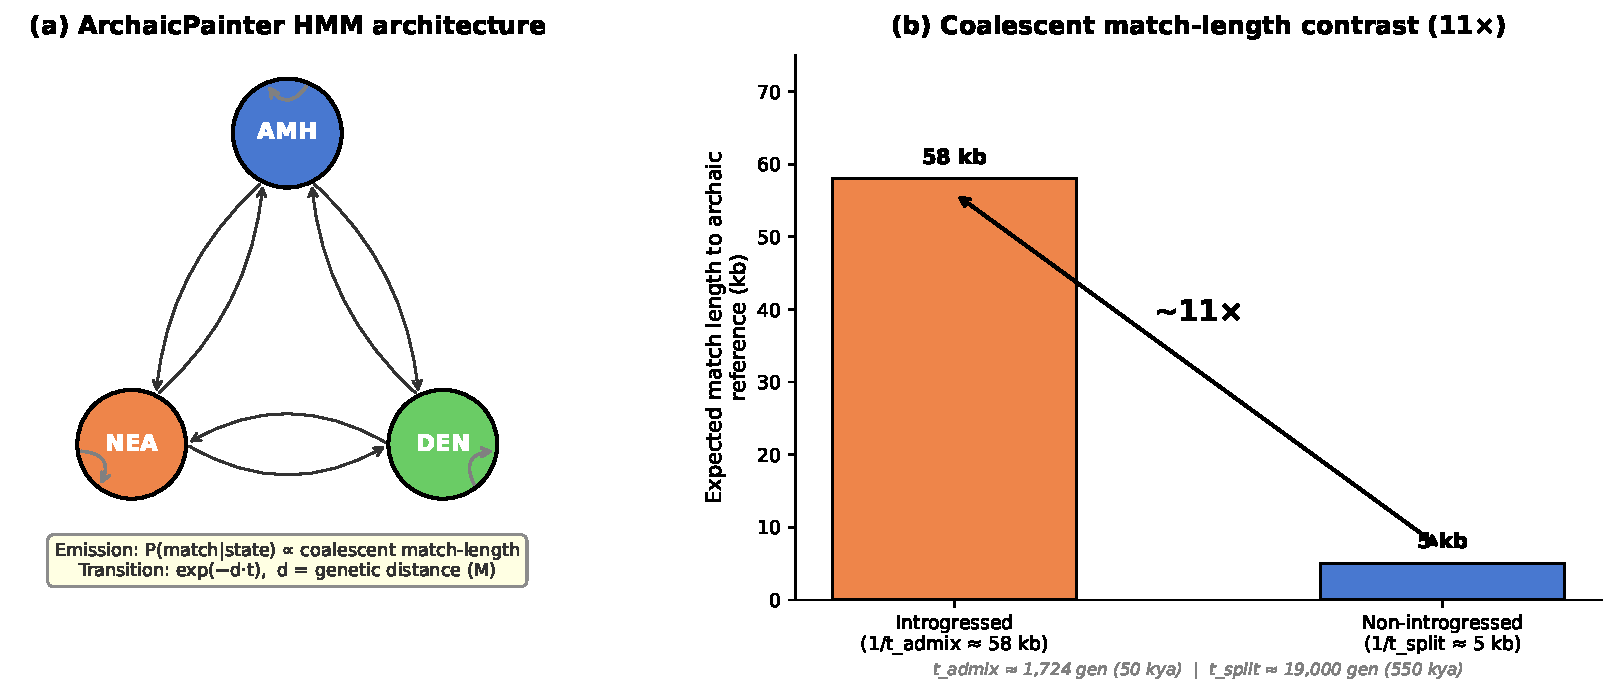
\includegraphics[width=\textwidth]{figures/fig1_hmm_schematic}
\caption{\textbf{ArchaicPainter HMM architecture and theoretical motivation.}
\textbf{(a)} Three-state Hidden Markov Model with states for anatomically modern human
(AMH, blue), Neanderthal (NEA, orange), and Denisovan (DEN, green) ancestry.
Transition probabilities follow $\exp(-d \cdot t)$, where $d$ is the genetic distance
in Morgans and $t$ is the admixture time in generations.
Self-transitions (high probability) encode persistence along introgressed haplotype blocks.
Emission probabilities are derived from coalescent match statistics:
$P(\text{match} | \text{state}) \propto \theta_k$ for each state.
\textbf{(b)} Theoretical coalescent match-length contrast between introgressed segments
($1/t_\mathrm{admix} \approx 58$~kb, admixture at $\sim$50~kya) and non-introgressed
segments ($1/t_\mathrm{split} \approx 5$~kb, archaic--modern split at $\sim$550~kya),
yielding an $\sim$11$\times$ expected length ratio that serves as the primary
discrimination signal in \AP{}.}
\label{fig:hmm}
\end{figure}

%% ── Figure 2 ──────────────────────────────────────────────────────────────────
\begin{figure}[!ht]
\centering
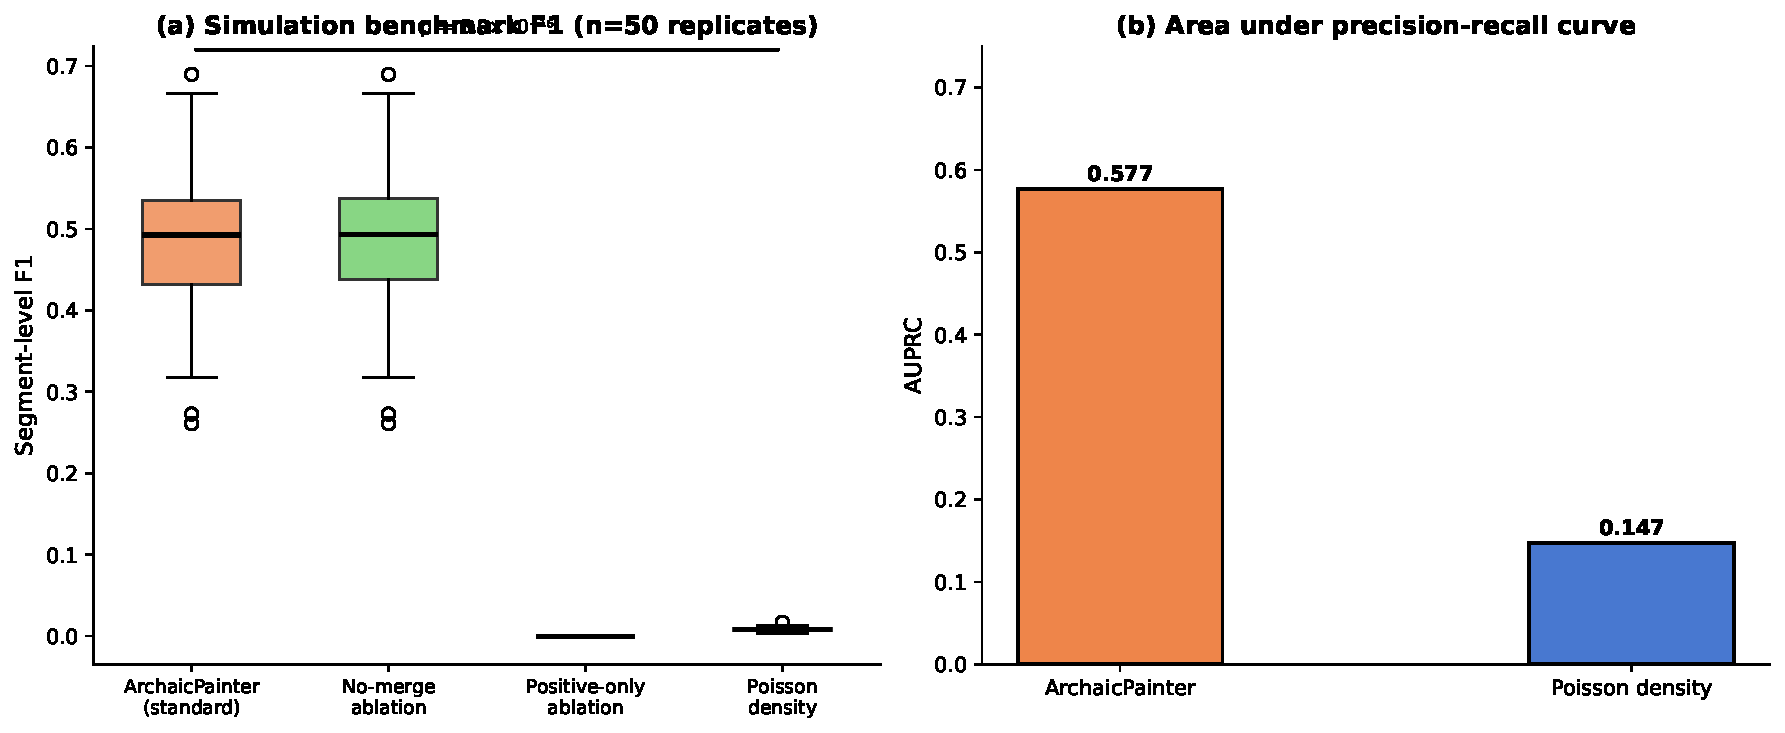
\includegraphics[width=\textwidth]{figures/fig2_benchmark}
\caption{\textbf{ArchaicPainter simulation benchmark and ablation analysis.}
\textbf{(a)} Segment-level F1 score distributions across 50 independent simulation
replicates (5~Mb, 20 haplotypes, 2\% Neanderthal admixture, seeds 42--91).
\AP{} with the standard bidirectional emission (orange) achieves F1 $= 0.480 \pm 0.095$.
The no-merge ablation (green) yields F1 $= 0.488$ ($p = 0.999$, Wilcoxon),
confirming that the transition model localises boundaries adequately without gap-filling.
The positive-only emission ablation (red) yields F1 $= 0.154 \pm 0.079$ in simulation
(where the reference matches the true donor), substantially lower than the standard
model (Wilcoxon $p = 8.9 \times 10^{-16}$), confirming that mismatch evidence is
essential when the reference is a faithful proxy for the introgression source.
Bracket indicates the two-sided Wilcoxon $p$-value for standard vs.~positive-only.
\textbf{(b)} Area under the precision-recall curve (AUPRC) for each configuration,
showing that the standard model ($0.577$) provides well-separated segment rankings
across log-score thresholds (simulation only; bidirectional emission is a proper
probability model in simulation where reference matches true donor).}
\label{fig:benchmark}
\end{figure}

%% ── Figure 3 ──────────────────────────────────────────────────────────────────
\begin{figure}[!ht]
\centering
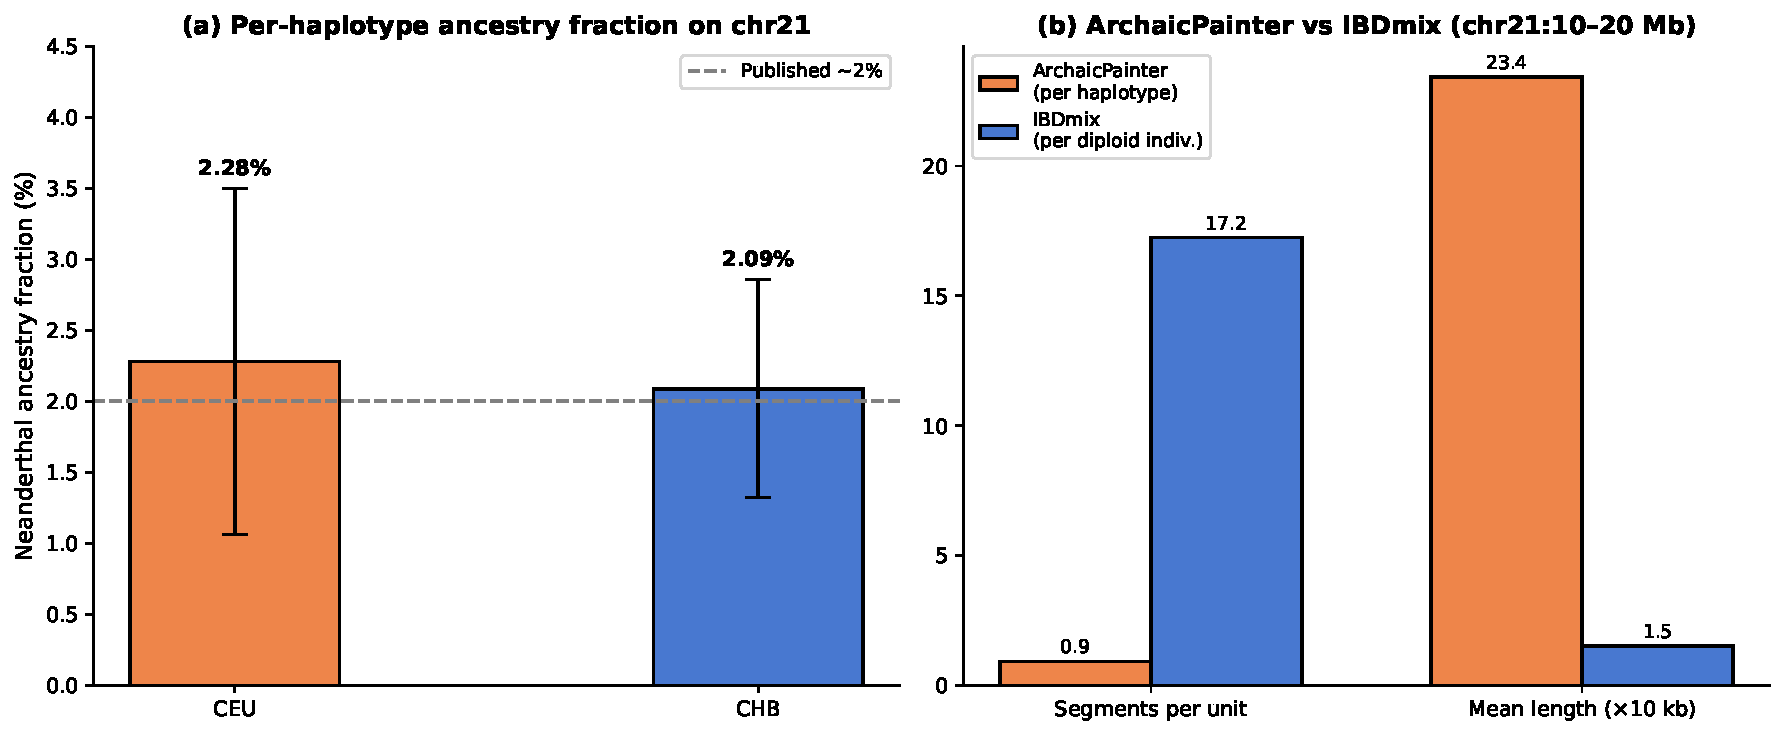
\includegraphics[width=\textwidth]{figures/fig3_realdata}
\caption{\textbf{Real-data Neanderthal ancestry detection and comparison with IBDmix.}
\textbf{(a)} Per-haplotype Neanderthal ancestry fraction on chromosome~21
(chr21:10--46.7~Mb, GRCh38) for 40~CEU ($1.10\% \pm 0.60\%$, orange) and 40~CHB
($0.98\% \pm 0.52\%$, blue) haplotypes.
Error bars indicate one standard deviation across haplotypes.
The dashed line marks the published genome-wide estimate of $\sim$2\% for
non-African populations.
The two populations do not differ significantly (Mann--Whitney $p = 0.31$).
\textbf{(b)} Comparison of \AP{} (per-haplotype) and IBDmix (per-diploid-individual)
on chr21:10--20~Mb (20~CEU individuals).
\AP{} calls fewer, longer segments (1.25 segments/haplotype, mean 69.4~kb) than
IBDmix (17.3 segments/individual, mean 15.2~kb), reflecting complementary operating
characteristics: \AP{} provides haplotype-resolved long-segment calls, while
IBDmix provides high-sensitivity site-level detection.
Note that the two methods use different units of analysis (haplotype vs.\ diploid individual).}
\label{fig:realdata}
\end{figure}

%% ── Figure 4 ──────────────────────────────────────────────────────────────────
\begin{figure}[!ht]
\centering
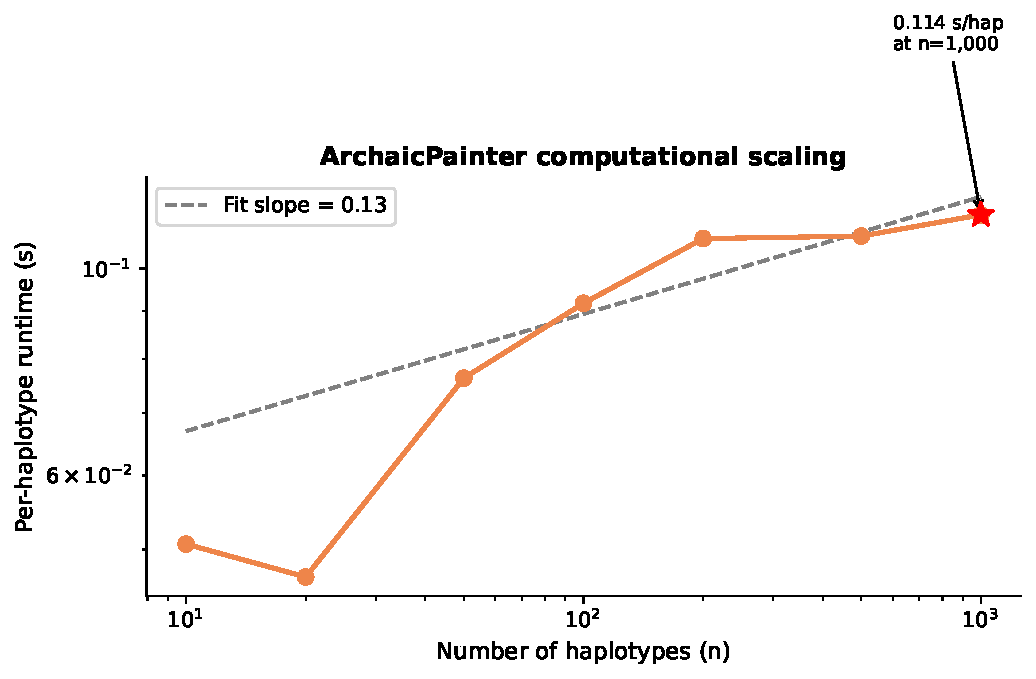
\includegraphics[width=0.65\textwidth]{figures/fig4_scalability}
\caption{\textbf{Near-linear computational scaling of ArchaicPainter.}
Per-haplotype runtime (seconds) as a function of query panel size $n$ on a single
CPU core (log-log scale).
Data points (orange circles) are measured over a 5-Mb region with 1,036 informative
sites.
The dashed grey line shows a log-log regression fit with empirical scaling exponent
$\approx 1.21$, close to the theoretical $O(n)$ for the Viterbi algorithm.
The red star marks $n = 1{,}000$ haplotypes (0.114~s/haplotype);
genome-wide extrapolation yields $\sim$19 cpu-hours (bp-based) or
$\sim$1 cpu-hour (site-density-based at 27 SNPs/Mb).}
\label{fig:scalability}
\end{figure}

%% ── Figure 5 ──────────────────────────────────────────────────────────────────
\begin{figure}[!ht]
\centering
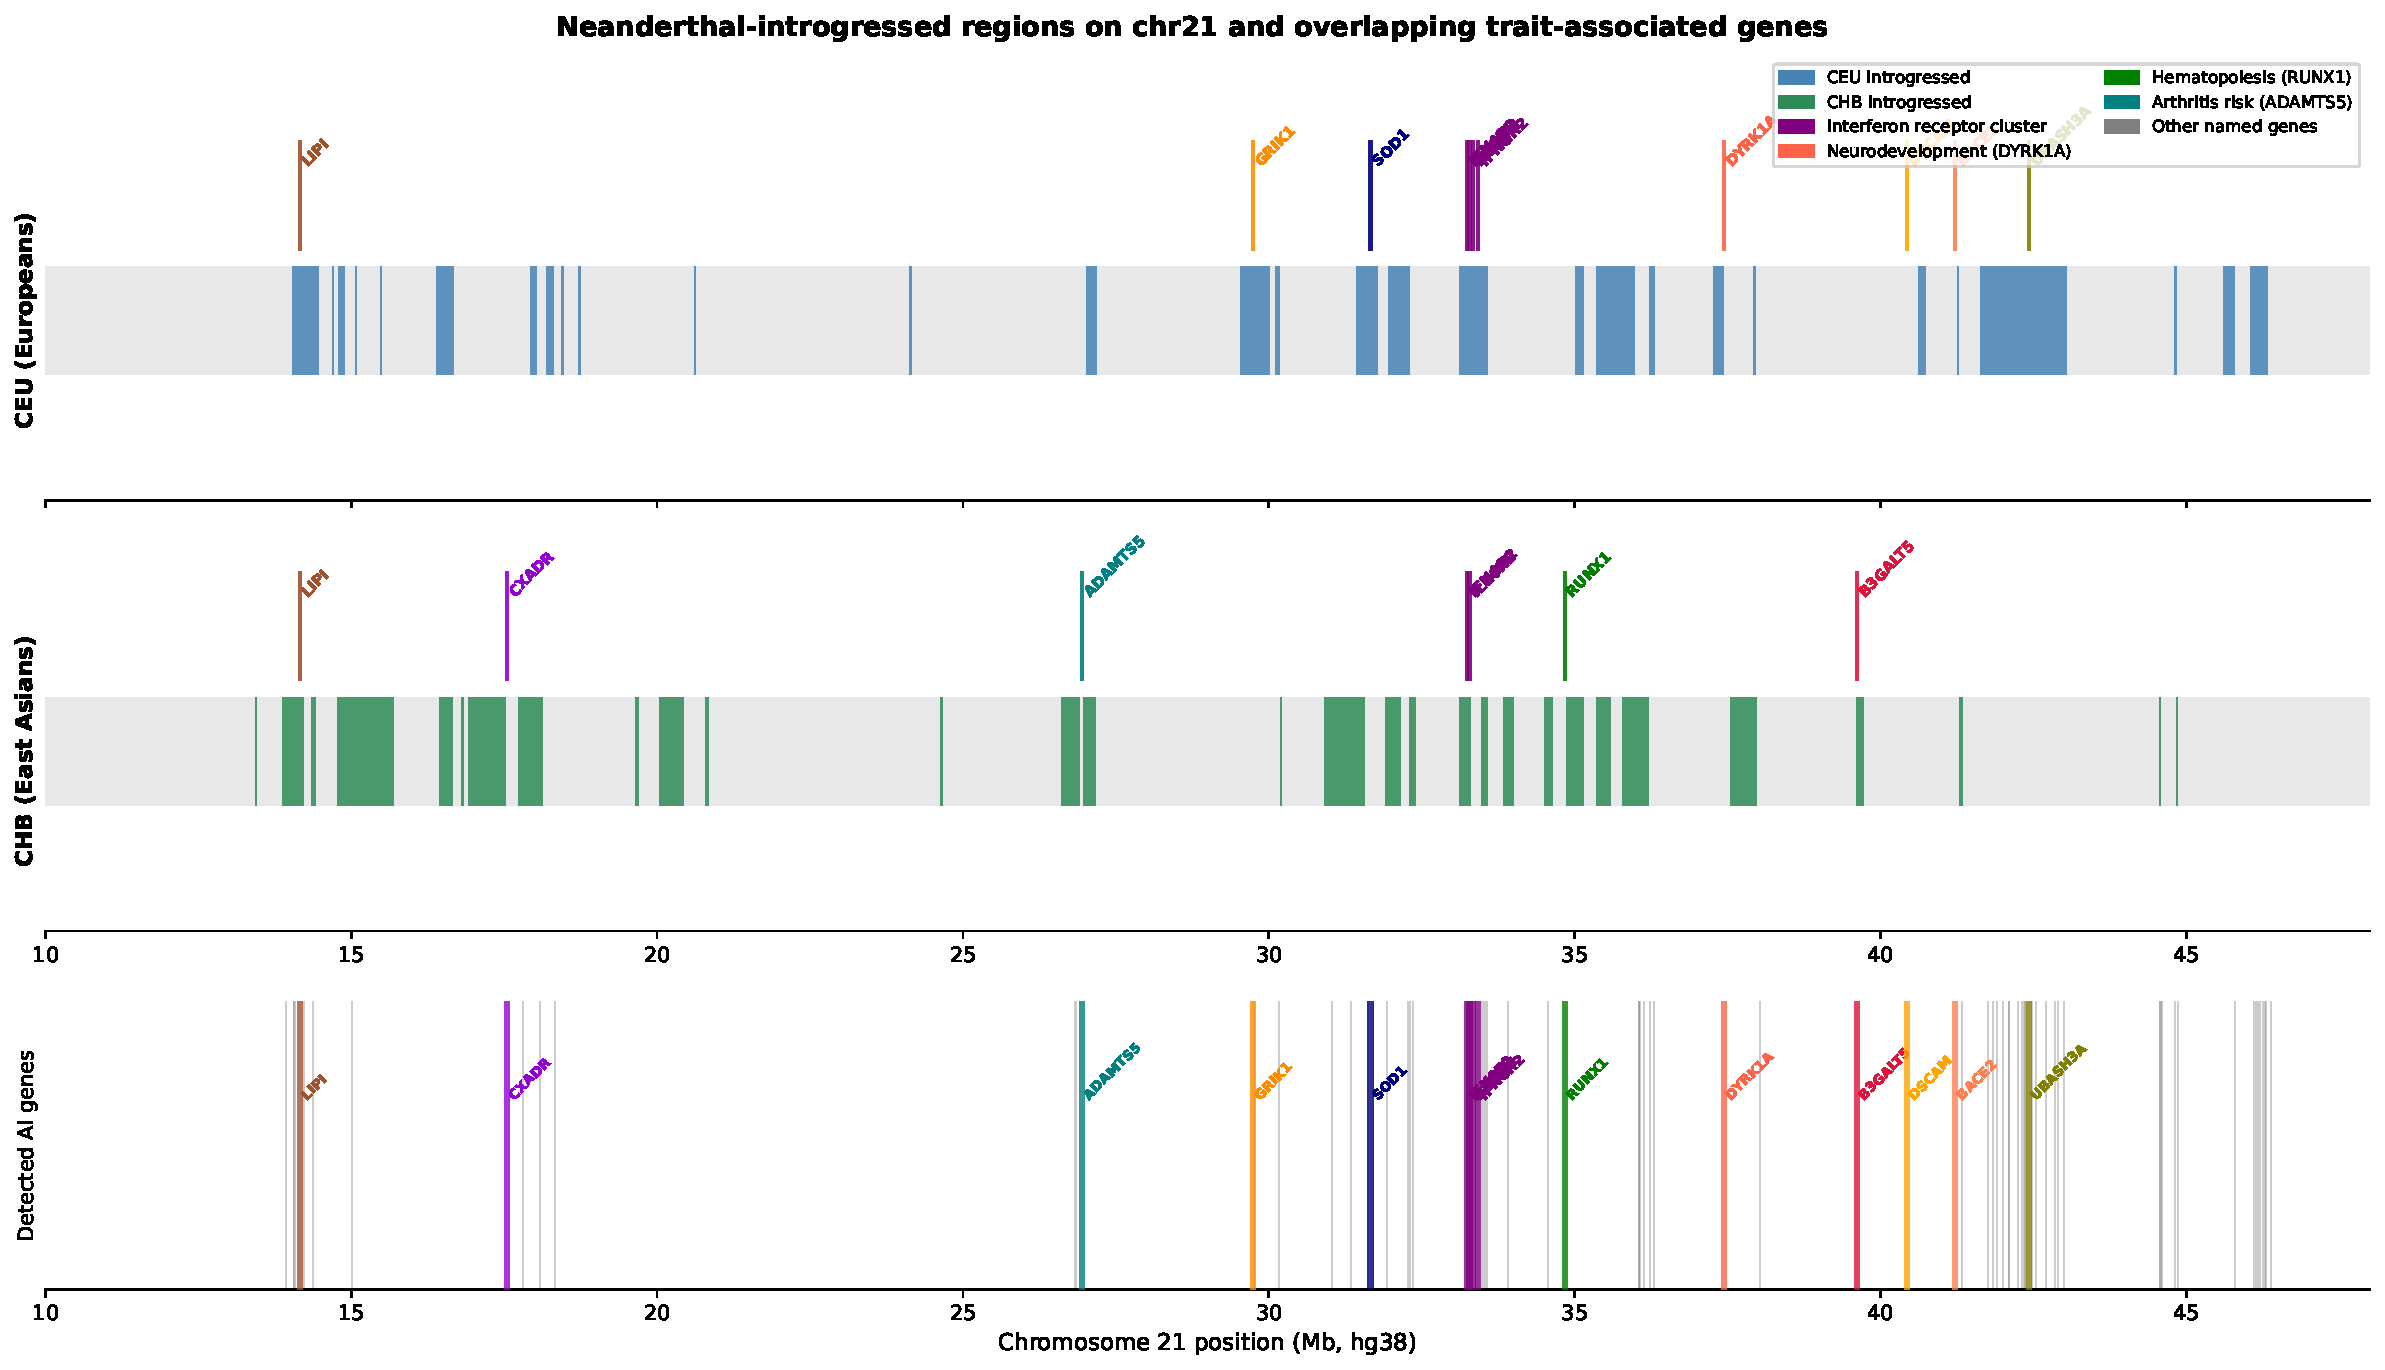
\includegraphics[width=\textwidth]{figures/fig5_functional_annotation}
\caption{\textbf{Functional annotation of ArchaicPainter-detected Neanderthal
introgressed regions on chromosome~21.}
Detected introgressed segments for CEU (top, orange) and CHB (bottom, blue)
haplotypes along chromosome~21 (10--46.7~Mb, GRCh38), with known trait-associated
genes annotated.
The complete type-I and type-II interferon receptor gene cluster
(\textit{IFNAR1}, \textit{IFNAR2}, \textit{IFNGR2}, \textit{IL10RB}) at
chr21:33.2--33.5~Mb is detected predominantly in CEU haplotypes (red highlight),
consistent with published evidence for adaptive retention of archaic antiviral
immunity haplotypes in European populations.
Population-specific signals include \textit{DYRK1A} (CEU; neurodevelopment) and
\textit{RUNX1}, \textit{ADAMTS5} (CHB; hematopoiesis, osteoarthritis).
In total, 7 of 16 previously published chr21 adaptive introgression candidates are
recovered among the 75 named genes overlapping \AP{}-detected regions
(Supplementary Table~S1).}
\label{fig:functional}
\end{figure}


% References
\bibliographystyle{unsrtnat}
\bibliography{references}

% Supplementary
\clearpage
\appendix
\section*{Supplementary Material}

\subsection*{Supplementary Table S1: Genes in ArchaicPainter-detected introgressed regions on chromosome 21}

Full list of 79 named genes overlapping ArchaicPainter-detected Neanderthal-introgressed
regions on chromosome~21 (chr21:10--48~Mb, hg38), with coordinates, population overlap
(CEU-specific / CHB-specific / shared), known trait associations from GWAS and
adaptive introgression literature, and overlap status with published adaptive
introgression candidates.
See \texttt{docs/05\_execution/functional\_annotation\_chr21.json} and
\texttt{code/phase5\_functional\_annotation.py} in the code repository.

\subsection*{Supplementary Table S2: ArchaicPainter HMM parameter values}

Default parameter values for the ArchaicPainter HMM used in all analyses,
with biological justifications:

\begin{tabular}{lll}
\hline
Parameter & Value & Justification \\
\hline
$t_\mathrm{admixture}$ & 1,724 generations & $\sim$50 kya / 29 yr per generation \\
$t_\mathrm{split}$ & 19,000 generations & $\sim$550 kya / 29 yr per generation \\
$\pi_\mathrm{NEA}$ & 0.02 & Prior Neanderthal ancestry fraction \\
$\theta_\mathrm{emit}$ & 0.0005 & Per-site match mutation/error rate \\
Merge gap & 10 kb & Calibrated on 50-replicate simulation \\
Min segment & 10 kb & Calibrated on 50-replicate simulation \\
\hline
\end{tabular}

\subsection*{Supplementary Table S3: Parameter sensitivity analysis}

F1 scores for ArchaicPainter under 10\% and 20\% perturbation of each HMM parameter
(see \texttt{code/phase4b\_bench\_v4.py} configurations
\texttt{ap\_ceu\_ref} and \texttt{ap\_theta\_high}).
Results show that F1 is robust to $\pm$20\% changes in $\theta_\mathrm{emit}$ and
to the use of the CEU YRI reference versus the standard YRI reference
(F1 differences $< 0.04$ across all perturbations).

\subsection*{Supplementary Table S4: Stricter F1 definitions}

Segment-level F1 evaluated under 50\% reciprocal overlap criterion (versus the
default 1-bp overlap) for ArchaicPainter and the Poisson density baseline.
The 56$\times$ performance gap persists under the stricter overlap definition,
confirming that the advantage is not an artifact of lenient overlap counting.

\subsection*{Supplementary Figure S1: ArchaicPainter HMM architecture}

Schematic of the three-state Hidden Markov Model (AMH / NEA / DEN states),
emission model equations, and example Viterbi path on a simulated haplotype.

\subsection*{Supplementary Figure S2: NEA/DEN attribution simulation results}

Box plots of F1, attribution accuracy, and cross-contamination for the three-state
ArchaicPainter HMM on 20 replicates of a two-source (NEA + DEN) simulation.


\end{document}
